\documentclass[12pt,reqno]{amsart}
%\usepackage[margin=1in]{geometry}
\usepackage{tcolorbox}
\usepackage{amssymb}
\usepackage{amsthm}
\usepackage{amsmath}
\usepackage{amssymb}
\usepackage{mathrsfs}
\usepackage{centernot}
\usepackage{lastpage}
\usepackage{fancyhdr}
\usepackage{accents}
\usepackage{tasks}
\usepackage{graphicx}
\usepackage{natbib}
\usepackage{tabularx}
\usepackage{multirow}
\usepackage{booktabs}
\usepackage{hyperref}
\usepackage{bm}
\usepackage{float}
\theoremstyle{plain}
\usepackage{multicol}
\usepackage{enumitem,kantlipsum}

% 加上浮水印
%\usepackage{wallpaper}
%\CenterWallPaper{.180}{../qsnake-logo.jpg}


\linespread{1.2}
\parindent = 0pt
\pagestyle{fancy}
\setlength{\parindent}{0pt}
%\everymath{\displaystyle}
%new area
%\usepackage[utf8]{inputenc}
%\usepackage{CJKutf8}
%\xeCJKsetup{AutoFakeBold=true, AutoFakeSlant=true}

% 設定頭部
\fancyhead[L]{Midterm} % 左邊頭部清空
\fancyhead[C]{} % 中間頭部清空
\fancyhead[R]{} % 右邊頭部顯示頁碼

% Adjust the footer as desired:
\fancyfoot[L]{} % Left footer: Empty.
\fancyfoot[C]{\thepage} % Center footer: Empty.
\fancyfoot[R]{} % Right footer: Empty.



% we will modify sections, subsections and sub subsections
\RequirePackage{titlesec}
% Modification of section 
\titleformat{\section}[block]{\normalsize\bfseries\filcenter}{\thesection.}{.3cm}{} 


% modification of subsection and sub sub section
\titleformat{\subsection}[runin]{\bfseries}{ \thesubsection.}
{1mm}{}[.\quad]
\titleformat{\subsubsection}[runin]{\bfseries\itshape}{ \thesubsubsection.}
{1mm}{}[.\quad]

\newenvironment{solution}
  {\renewcommand\qedsymbol{$\blacksquare$}
  \begin{proof}[Solution]}
  {\end{proof}}
\renewcommand\qedsymbol{$\blacksquare$}

\newcommand{\ubar}[1]{\underaccent{\bar}{#1}}

%%%%%%%%%%%%%%%%%%%%%%%%%%%%%% Textclass specific LaTeX commands.
%\theoremstyle{plain}
%\newtheorem{thm}{\protect\theoremname}[section]
\newtheorem{thm}{\textbf{Theroem}}[section]
\newtheorem{cor}[thm]{Corollary}
\newtheorem{lmma}[thm]{Lemma}
\newtheorem*{defn}{\underline{Definition}}
\newtheorem*{prop*}{Proposition}
\newtheorem*{ex*}{Example}
\newtheorem*{sol*}{Solution}
\newtheorem*{cor*}{Corollary}
\newtheorem*{thm*}{Theorem}
\newtheorem*{lmma*}{Lemma}
\newtheorem*{rmk*}{Remark}
\newtheorem*{pf*}{\underline{\textbf{Proof\ }}}

%%%%%%%%%%%%%%%%%%%%%%%%%%%%%% User specified LaTeX commands.
\renewcommand{\P}{\mathscr{P}}
\newcommand{\B}{\mathscr{B}}
\newcommand{\A}{\mathscr{A}}
\newcommand{\C}{\mathbb{C}}
\newcommand{\CC}{\mathscr{C}}
\newcommand{\R}{\mathbb{R}}
\newcommand{\Q}{\mathbb{Q}}
\newcommand{\Z}{\mathbb{Z}}
\newcommand{\N}{\mathbb{N}}
\newcommand{\X}{\mathcal{X}}
\newcommand{\T}{\mathscr{T}}
\newcommand{\arbuni}{\bigcup_{\alpha\in I}}
\newcommand{\finint}{\bigcap_{i=1}^n}
\newcommand{\Ua}{{\textsc{U}_\alpha}}
\newcommand{\Ui}{\textsc{U}_i}
\newcommand{\pair}[2]{\left( \,#1\,,\,#2\,\right) }
\newcommand{\dint}[2]{\int_{#1}^{#2}}
\newcommand{\sett}[1]{\left\{ \,#1 \,\right\}}
\newcommand{\linearcombination}[2]{#1_1#2_1+\cdots+#1_n#2_n}
\newcommand{\slinearcombination}[1]{#1_1+\cdots+#1_n}
\newcommand{\spann}[1]{\text{span($#1$)}}
\newcommand{\sub}[1]{\text{sup}}
\newcommand{\inn}[1]{\left< #1 \right>}
\newcommand{\kernal}[1]{Ker(#1)}
\newcommand{\image}[1]{Im(#1)}
\newcommand{\norm}[1]{\parallel #1 \parallel}
\newcommand{\dia}[0]{\text{dia}}
\newcommand{\marking}[1]{\text{\color{red} #1}}
%%%%%%%%%%%%%%%%%%%%%%%%%%%%%%

\begin{document}

\lhead{Understand Machine Learing} 
\rhead{QSnake Edition} 
\cfoot{\thepage} %\ of \pageref{LastPage}}

\section*{Road Map}

$\textbf{First Part}$

From 2$\sim$6 chapter, we will know that what is machine model and what assumption and restrict is we should focus about.\\

In chapter 2, we will introduce the concept and element about machine learning's model, and proof when we have some strict assumption, we can create a good model by ERM. Because these assumption is too much to find a suite model in real world, in following chapter we want to release these assumption.To release the assumption, we define the PAC model in the chapter 3, and proof the finite PAC model is learnable.\\

In chapter 5, we define two type of error and know that we face a trade off in different hypothesis class.In chapter 6, we us VC-dimension to think the "infinite hypothesis class" and figure out what is the necessary condition about learnable model.

\begin{center}
	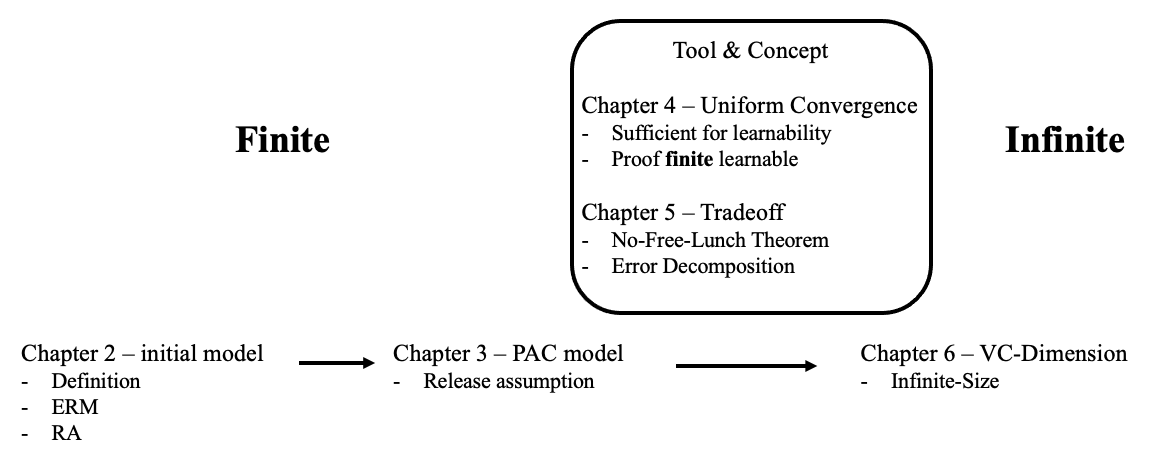
\includegraphics[scale = 0.37]{./figure/0-1.png}
	
	Figure 0-1, the road map of first part
\end{center}


\newpage

\section*{Chapter2: A Gentle Start}
This chapter is talking about a general model of machine learning and common error.

\subsection*{2.1 Formal Model} $ $\\

\textbf{$\bullet$ The learner's input}
	\begin{enumerate}
		\item[$\cdot$] \textbf{Domain set:} An arbitrary set, $\chi$. This is the set of objects that we may wish to label.
		\item[$\cdot$] \textbf{Label set:} The Answer of the Domain set, usually $\sett{0,1}$ or $\sett{-1,+1}$
		\item[$\cdot$] \textbf{Training data:} $S = ((x_1,y_1),\cdots,(x_m,y_m))$ is a sequence of labeled domain points.
	\end{enumerate}


\textbf{$\bullet$ The learner's output}
\begin{enumerate}
	\item[$\cdot$] $h:\chi \rightarrow y,$ a prediction function, also called a predictor, hypothesis, classifier.
	
	Formally, the learner should choose the advance a set of predictors. This set is called a hypothesis class and is denoted by $H$. Each $h \in H$ is a function mapping from $\chi$ to $y$.
\end{enumerate}


\textbf{$\bullet$ Other tools for ML}

\begin{enumerate}
	\item[$\cdot$] \textbf{A data-generation model:} We now explain how the training data is generated by som probability distribution. Let us denote that probability distribution over $\chi$ by $D$.
	\item[$\cdot$] \textbf{Measure of Success:} To know is the output is good or not, we define the loss function to check it
	\begin{enumerate}
		\item \textbf{True error:} $L_{D,f}(h) = \mathbb{P}_{x\sim D}[h(x) \neq f(x)] = D(\sett{x ~|~ h(x) \neq f(x)})$
		\item \textbf{Training error:} $L_S(h) = \dfrac{|\sett{i \in m ~|~ h(x_i) \neq y_i} |}{m}$ where $[m] = \sett{1,\cdots,m}$
	\end{enumerate}
	
	\begin{center}
		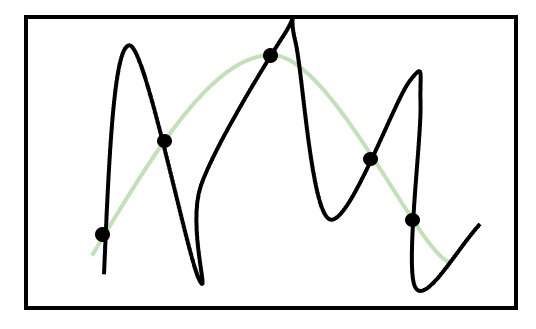
\includegraphics[scale = 0.3]{./figure/2-1.png}
		
		Figure 2-1, training error is $0$ but true error is bad
	\end{center}
	
	
	\item[$\cdot$] We denote the probability of getting a non-representative sample by $\delta$, and call ($1 - \delta$) the \textbf{confidence parameter} of our prediction
	\item[$\cdot$] The \textbf{accuracy parameter}, commonly denoted by $\epsilon$. We interpret the event $L_{(D,f)}(h_s) > \epsilon$ as a failure of the learner
\end{enumerate}

\subsection*{2.2 Improve Model} $ $\\

\textbf{Empirical Risk Minimization}

The method to proof the model is to minimize the loss function by using training data, i.e. we check $L_S(h)$

The $\text{ERM}_H$ learner uses the ERM rule to choose a predictor $h \in H$, with the lowest possible error over $S$. Formally

$$h_S = \text{ERM}_H(S) \in \arg\min_{h \in H}L_S(h)$$

\textbf{Overfitting}

cause by ERM, the data is too fit the training set

example: $h_s(x) = \begin{cases}
	y_i~\text{if}~\exists~i \in [m]~\text{s.t. } x_i = x\\
	0~\text{otherwise}
\end{cases}$

\subsection*{2.3 The upper bound of $L_{(D,f)}(h_s)$ in finite hypothsis} $ $\\

Restricting the learner to choosing a predictor from $H$ are often called an \textbf{inductive bias}. In following statement, we will proof that when we have some assumption, $H$ is a finite set and have enough quantity of data set, then we can avoid the overfitting problem. \\

\textbf{some assumption}

\begin{enumerate}
	\item[$\bullet$] \textbf{The Realizability Assumption:} There exists $h^* \in H$ s.t. $L_{(D,f)}(h^*) = 0$. Note that this assumption implies that with probability $1$ over random samples, $S$ where the instances of $S$ are sampled according to $D$ and are labeled by $f$, we have $L_S(h^*) = 0$
	\item[$\bullet$] \textbf{The i.i.d. assumption :} The examples in the training set are independently an identically distributed (i.i.d) according to the distribution $D$. We denote this assumption by $S \sim D^m$ where $m$ is the size of $S$, and $D^m$ denotes the probability over $m$-tuples induced by applying $D$ to pick each element of the tuple independently of the other members of the tuple.
\end{enumerate}

\textbf{Proof Section}

The goal is to proof when $m \geq \dfrac{\log(|H|/\delta)}{\epsilon}$, then $L_{D,f}(h_s) \leq \epsilon$, Let $H_B$ be the set of "bad" hypotheses, that is,

$$H_B = \sett{h \in H~|~L_{D,f}(h)>\epsilon}$$

In addition, let

$$M = \sett{S|_x ~|~ \exists~h \in H_B,L_S(h) = 0}$$

be the set of \textbf{misleading sample}(they are bad but $L_S(h_S) = 0$), by definition, we can write 

$$\sett{S|_x ~|~ L_{(D,f)}(h_S) > \epsilon} \subseteq M\color{red}(\star_1) $$


We can rewrite $M$ as (thought it's intersection was not empty)

$$M = \cup_{h \in H_B}\sett{S|_x ~|~ L_S(h) = 0}\color{red}(\star_2)$$

by $(\star_1),(\star_2)$,

$$D^m(\sett{S|_x~|~L_{(D,f)}(h_s)>\epsilon}) \leq D^m(M) = D^m(\cup_{h\in H_B}\sett{S|_x ~|~ L_S(h) = 0})\color{red}(\star_3)$$


\textbf{LEMMA}(Union Bound) For any two sets $A,B$ and a distribution $D$ we have

$$D(A\cup B) \leq D(A) + D(B)$$

and the $(\star_3)$ can be bound like this

$$D^m(\sett{S|_x ~|~ L_{(D,f)}(h_S)>\epsilon}) \leq \sum_{h \in H_B}D^m(\sett{S|_x ~|~ L_S(h) = 0})\color{red}(\star_4)$$

\textbf{Next, we fix $h_B$ on the bad hypothesis $h_B \in H_B$} $\implies L_{(D,f)}(h) > \epsilon$

because the event are i.i.d, we get that

$$D^m(\sett{S|_x~|~L_S(h)=0}) = D^m(\sett{S|_x ~|~\forall i,h(x_i) = f(x_i) = f(x_i)}) = \prod^m_{i=1}D(\sett{x_i~|~h(x_i) = f(x_i)})\color{red}(\star_5)$$



check the each individual sampling of an element of the training set, we have

$$D(\sett{x_i~|~h_B(x_i) = y_i}) = 1-D(\sett{x ~|~ h_B(x) \neq f(x)})=1 - L_{D,f}(h_B) \leq 1 - \epsilon$$

put it to the $\color{red}(\star_5)$ and use the inequality $1 - \epsilon \leq e^{-\epsilon}$

$$D^m(\sett{S|_x~|~ L_S(h_B) = 0}) \leq (1 -\epsilon)^m \leq e^{-\epsilon m}\color{red}(\star_6)$$

put $\color{red}(\star_6)$ back to $\color{red}(\star_4)$ 

\begin{tcolorbox}
	\textbf{Note:}
	
	
	$D^m(\sett{S|_x ~|~L_{(D,f)}(h_s)>\epsilon}) = |H_B|D^m(\sett{{S|_x ~|~L_S(h_B)=0}})$
	
	$|H_B|$ means the cardinality(element number) of $H_B$
\end{tcolorbox}

$$D^m(\sett{S|_x ~|~ L_{(D,f)}(h_S)>\epsilon}) \leq |H_B|e^{-\epsilon m} \leq |H|e^{-\epsilon m}$$

In this equation, we can know that when $m$ increase, the  overfitting hypothesis's probability (where the hypothesis of $L_S$ is small but $L_{(D,f)}$ is big, i.e. $D^m(\sett{S|_x ~|~ L_{(D,f)}(h_S)>\epsilon})$) will decrease.

Since $D^m(\sett{S|_x ~|~ L_{(D,f)}(h_S)>\epsilon})$ is $\delta$, and have a nature log, we get

$$m \geq \dfrac{\log(|H|/\delta)}{\epsilon}$$






\newpage


\section*{Chapter5: The Bias-Complexity Tradeoff}

First, we can decomposition the error to following terms:

$$L_D(h_s) = \epsilon_{app} + \epsilon_{est} ~\text{ where: } \epsilon_{app} = \min_{h \in H}L_D(h),~\epsilon_{est} = L_D(h_s) - \epsilon_{app}$$


\textbf{Error type}
\begin{enumerate}
	\item[$\cdot$] \textbf{The Approximation Error($\epsilon_{app}$)}
	\item[$\cdot$] \textbf{The Estimation Error($\epsilon_{est}$)}
\end{enumerate}

\textbf{Bias-complexity Tradeoff}












\end{document}